% Ehemals Entwurfsskizze.pdf
\section{Entwurfsskizze}\label{sec:entwurfsskizze}
\textit{Abschlussprojekt Modul \glqq Assemblerprogrammierung\grqq{} von Konstantin Blechschmidt \& Tim M.\ Kretzschmar}

% TODO v2.0.0: Teile dieses Entwurfs sind ueberholt (siehe Kommentare in
% funktionalitaet.tex).
Unser Programm kann in 2 Hauptbereiche mit je 2 Unterbereichen aufgeteilt werden.

\begin{description}[labelwidth=1cm,leftmargin=1.4cm,style=nextline]
    \item[I.\ Verschlüsselung]
        \begin{enumerate}[label=\alph*),noitemsep,topsep=0pt]
            \item graphische Ein-/Ausgabe Klartext und Ausgabe des Chiffretextes im Bildschirm + Schlüssel
            \item Abarbeitung der Verschlüsselung unter Zuhilfenahme der \asm{PROC}s aus der \asm{VERS.asm}
        \end{enumerate}
    \item[II.\ Entschlüsselung]
        \begin{enumerate}[label=\alph*),start=3,noitemsep,topsep=0pt]
            \item graphische Ein-/Ausgabe Chiffretext und Ausgabe des Klartextes im Bildschirm + Schlüssel
            \item Abarbeitung der Entschlüsselung unter Zuhilfenahme der \asm{PROC}s aus der \asm{ENTS.asm} und teilweise \asm{VERS.asm}
        \end{enumerate}
\end{description}

\begin{figure}[!htbp]
    \centering
    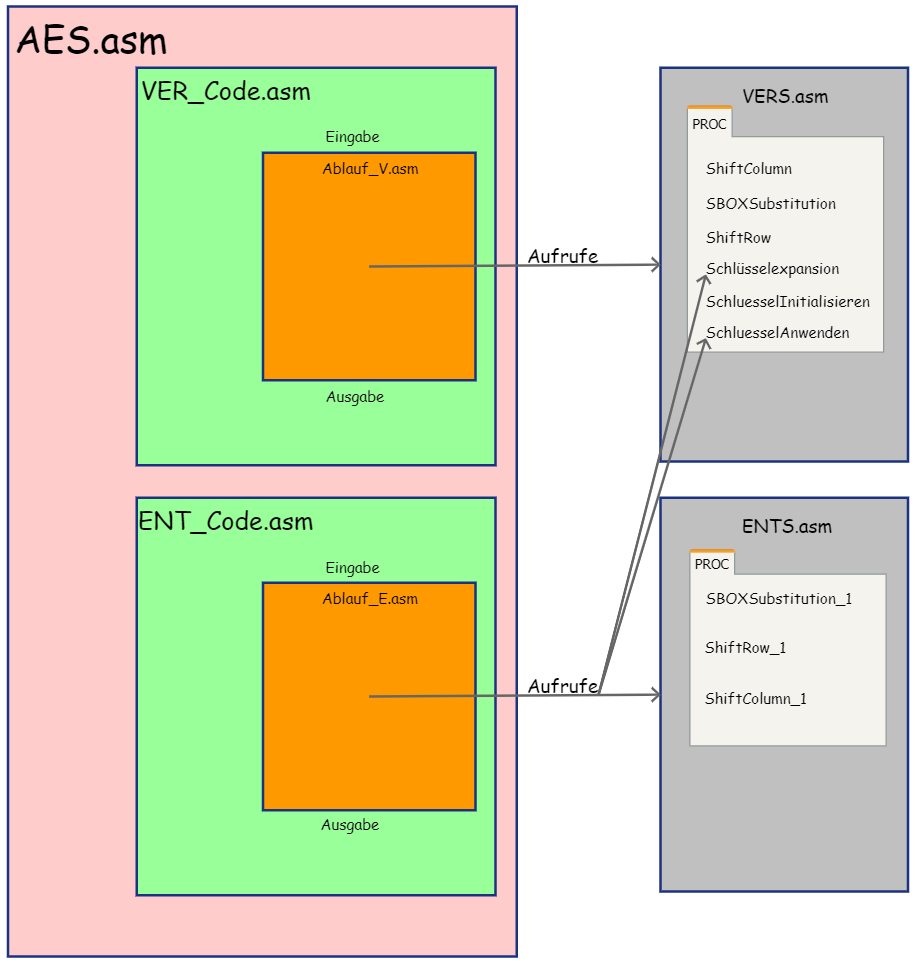
\includegraphics[height=0.5\textheight,keepaspectratio]{images/entw_zusammenspiel.png}
    \caption{Entwurf: Zusammenspiel der ASM-Dateien}
    \label{fig:entw-zusammenspiel}
\end{figure}

\begin{figure}[!htbp]
    \centering
    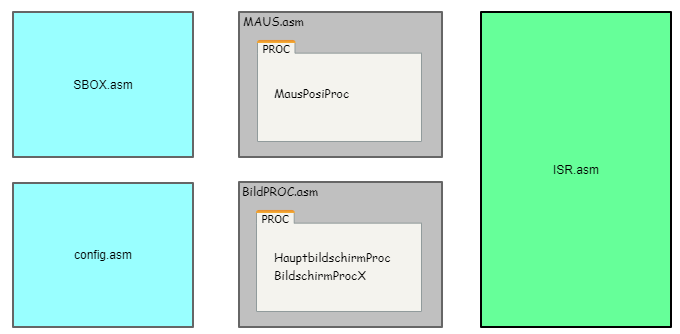
\includegraphics[width=0.8\textwidth]{images/entw_uebersicht.png}
    \caption{Entwurf: Übersicht der weiteren ASM-Dateien}
    \label{fig:entw-uebersicht}
\end{figure}

Jede \asm{PROC} und jeder Programmteil ist im Kopfbereich der ASM-Datei und im Handbuch näher beschrieben. Eine möglichst klare Erläuterung der jeweiligen Befehlszeilen befindet sich ebenfalls in den ASM-Dateien als Kommentar.

% TODO v2.0.0: Die folgenden zwei Absaetze beschreiben den Stand 1.x (inverse
% ShiftColumn nicht lauffaehig, AES-konformer Code auskommentiert). Seit 2.0.0
% sind ShiftColumn/ShiftColumn_1 (MixColumns + Inverse) implementiert; ob sie in
% Ablauf_V.asm/Ablauf_E.asm aktiviert sind, bitte im Quelltext pruefen.
Leider können wir die echte Version von AES nicht vorzeigen, da es uns nicht möglich war, die inverse \asm{ShiftColumn} zu implementieren. Die Verrechnung mit der inversen C-Matrix aus E, D, B, 9 (alles hexadezimale Werte) haben wir programmiert, aber das Ergebnis war nach mehreren Versuchen immer noch falsch.

Aus diesem Grund befindet sich unter dem Quelltext von der \asm{Ablauf_E.asm} und \asm{Ablauf_V.asm} der auskommentierte Code, der für den Ablauf nach AES-Standard vorgesehen wäre. Der nicht auskommentierte Code darüber soll die verfügbaren und nutzbaren Aspekte von AES anwenden, also dem Nutzer eine Verschlüsselung bieten, die AES-ähnlich ist. Die schon kompilierte \asm{AES.EXE} beinhaltet diese AES-ähnliche Umsetzung.

Bezüglich der Variablen existieren die \asm{config.asm} und \asm{SBOX.asm}. Dort kann in den Kommentaren Näheres zu deren Einsatz erfahren werden, sowie eine Übersicht im Handbuch unter dem entsprechenden Absatz (Abschnitt~\ref{sec:asm-dateien}) eingesehen werden.
